\documentclass[tikz]{standalone}
\usetikzlibrary{bayesnet, arrows.meta}

\begin{document}
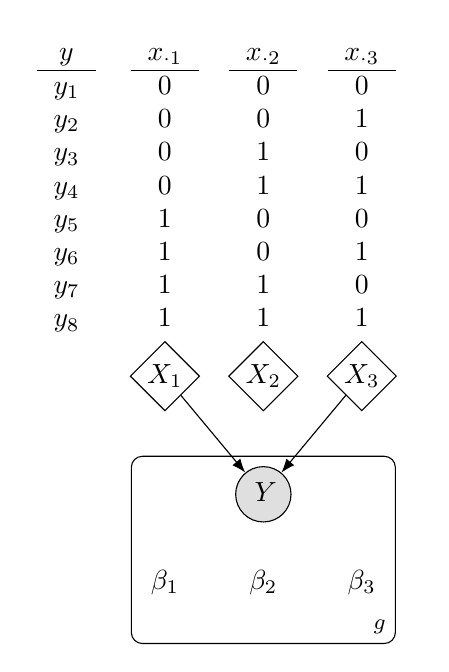
\begin{tikzpicture}


% GLOBAL SETTINGS
\newcommand{\p}{3}
\newcommand{\Xstyle}{det}
\newcommand{\Bstyle}{}
\newcommand{\mybeta}{\(\beta_1\)}

% SHARED CODE
\newlength{\xdist}
\setlength{\xdist}{1.25cm}
\newlength{\ydist}
\setlength{\ydist}{1.5cm}
\pgfkeys{/tikz/every path/.style={->, -{Latex[length=5pt]}}} % draw arrowheads
% X
\path (-2\xdist,\ydist) foreach \j in {1,...,\p} {
++(\xdist,0) node[\Xstyle] (X\j) {\(X_\j\)}
+(0,-1.75\ydist) coordinate (b\j) 
};
% beta
\path (-2\xdist,\ydist) foreach \j in {2,...,\p} {
(b\j) node[\Bstyle] (B\j) {\(\beta_{\j }\)}
};
\node[\Bstyle] (B1) at (b1) {\mybeta};
% helper coordinates
\path
(b1) +(-0.6\xdist,-0.0\ydist) coordinate (bL)
(b\p) +(+0.6\xdist,-0.0\ydist) coordinate (bR) ;
% Y
\node[obs] (Y) at (0,0) {\(Y_{}\)};



% EDGES & PLATE
\foreach \j in {1,3} { \draw (X\j) -- (Y) ;}
\plate {v-plate} {(Y) (B1) (B\p)} {\(g\)};

% DATA
%
\path (X1) +(-\xdist,0.25\ydist) node[anchor=south] {
\begin{tabular}{c}
\(y_{}\) \\ \hline
\(y_1\) \\ \(y_2\) \\ \(y_3\) \\ \(y_4\) \\ \(y_5\) \\ \(y_6\) \\ \(y_7\) \\ \(y_8\) \\
\end{tabular} } ;
%
\path (X1) +(0,0.25\ydist) node[anchor=south] {
\begin{tabular}{c}
\(x_{\cdot 1}\) \\ \hline
0 \\ 0 \\ 0 \\ 0 \\ 1 \\ 1 \\ 1 \\ 1 \\
\end{tabular} } ;
%
\path (X2) +(0,0.25\ydist) node[anchor=south] {
\begin{tabular}{c}
\(x_{\cdot 2}\) \\ \hline
0 \\ 0 \\ 1 \\ 1 \\ 0 \\ 0 \\ 1 \\ 1 \\
\end{tabular} } ;
%
\path (X3) +(0,0.25\ydist) node[anchor=south] {
\begin{tabular}{c}
\(x_{\cdot 3}\) \\ \hline
0 \\ 1 \\ 0 \\ 1 \\ 0 \\ 1 \\ 0 \\ 1 \\
\end{tabular} } ;

\end{tikzpicture}
\end{document}
